% \usepackage{xcolor}
% \usepackage{afterpage}
% \usepackage{pifont,mdframed}
% \usepackage[bottom]{footmisc}

\makeatletter
\gdef\this@inputfilename{input.txt}
\gdef\this@outputfilename{output.txt}
\makeatother

\newcommand{\inputfile}{\texttt{input.txt}}
\newcommand{\outputfile}{\texttt{output.txt}}

\newenvironment{warning}
  {\par\begin{mdframed}[linewidth=2pt,linecolor=gray]%
    \begin{list}{}{\leftmargin=1cm
                   \labelwidth=\leftmargin}\item[\Large\ding{43}]}
  {\end{list}\end{mdframed}\par}
  
\begin{tabular}{cl}
\begin{minipage}[t]{2cm}
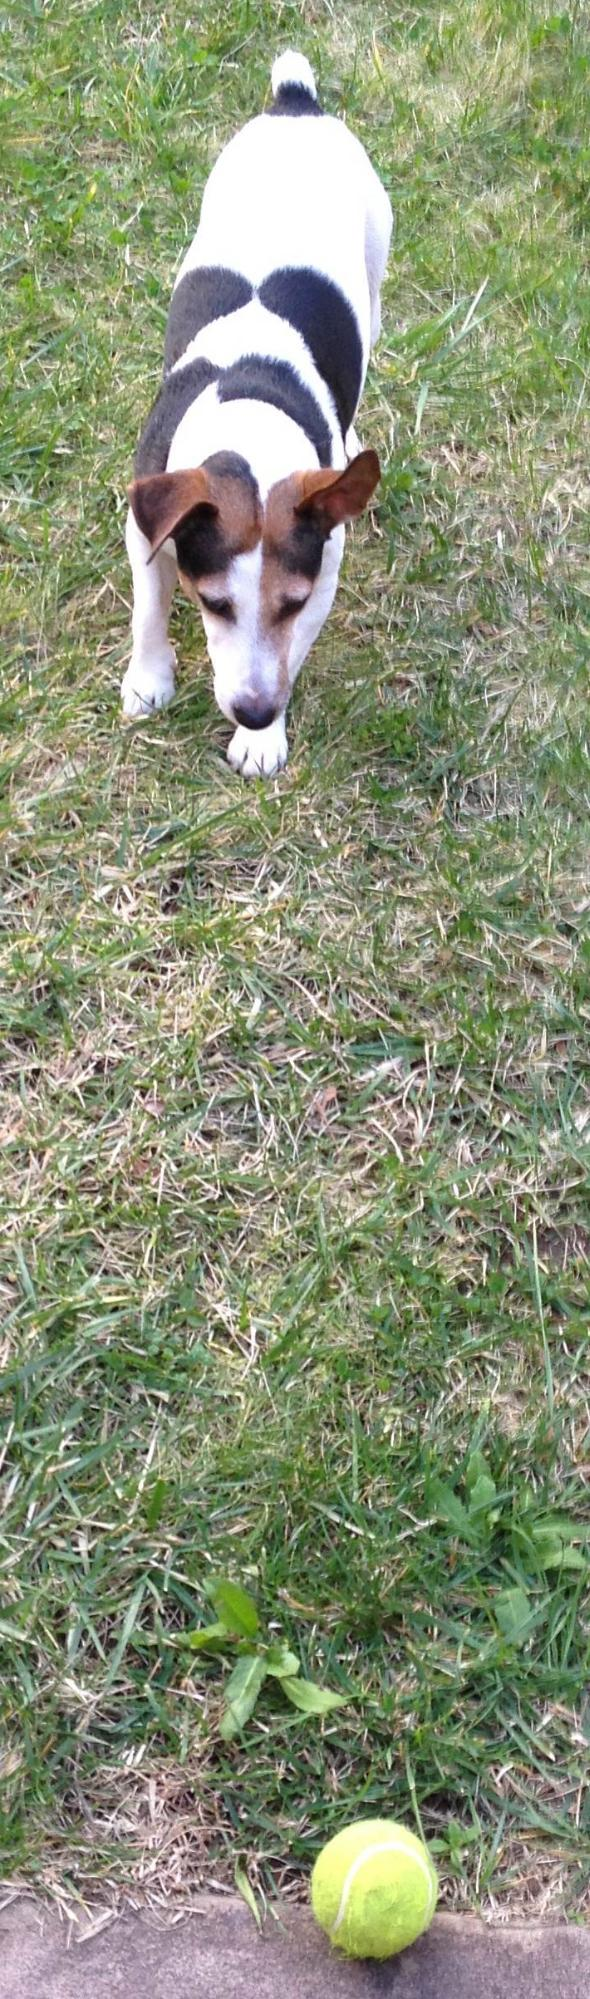
\includegraphics[width=2cm]{mojito.jpg}\\
\vspace{0.1cm}
\end{minipage} 
&
\begin{minipage}[b]{0.8\textwidth}
Mojito, il jackrussell di Monica, è ormai diventato la mascotte dei Probabili Olimpici, i ragazzi che sono candidati a rappresentare l’Italia alle Olimpiadi Internazionali di Informatica 2015 a Astana, Kazakistan. Negli allenamenti a Volterra, Mojito gioca a palla con i ragazzi nel prato: lui porta la pallina al ragazzo più vicino che la calcia via; a quel punto Mojito rincorre la palla, l’acchiappa e la porta di nuovo al ragazzo che ha più vicino… e così via!
Possiamo rappresentare questo gioco con una griglia: supponendo di avere tre ragazzi che giocano con Mojito, rappresentiamo la loro posizione nella griglia, rispettivamente, con R1, R2 e R3. Tutti i ragazzi sono piuttosto metodici, e ogni volta che tirano la palla questa finisce sempre nella stessa posizione (a seconda di chi tira!): sulla griglia indichiamo con P1 il punto in cui finisce la palla tirata da R1, P2 il punto in cui finisce la palla tirata da R2, ecc... La posizione iniziale di Mojito, con la palla, è rappresentata nella griglia da una M. Mojito misura la distanza come il minimo numero di spostamenti orizzontali e/o verticali per andare da una casella a un’altra.
\end{minipage}
\end{tabular}
\begin{center}
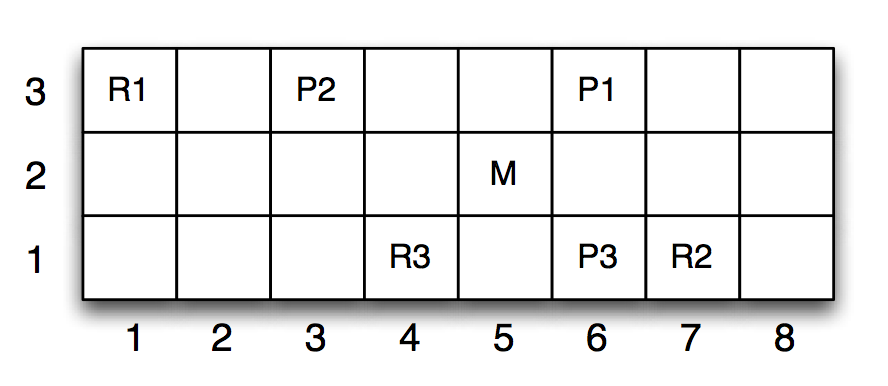
\includegraphics{griglia.png}
\end{center}

Per esempio, consideriamo la griglia qui sopra, di dimensione $8 \times 3$. All’inizio Mojito si trova, insieme con la palla, nella casella $(5,2)$; il ragazzo più vicino è R3, nella posizione $(4,1)$, che dista due caselle da lui; il gioco inizia:
\begin{itemize}
\item Mojito porta la palla a R3, che la tira nella casella (6,1); 
\item a questo punto Mojito, presa la palla, la porta a R2, nella casella (7,1), che è il più vicino a lui; da qui la palla viene tirata nella casella (3,3); 
\item Mojito recupera la palla e la porta a R1, nella  casella (1,3); R1 tira la palla nella casella (6,3); 
\item da qui in poi saranno solo R1 e R2 a giocare, visto che quando tira R1 poi Mojito porta la palla a R2 e viceversa.
\end{itemize}

Notiamo che, nel caso appena descritto, tutti e tre i ragazzi hanno giocato (anche se R3 ha toccato palla solo una volta). Se Mojito ha due o più ragazzi alla stessa distanza, sceglie quello che ha la coordinata $X$ (orizzontale) minore e, se ve ne sono due o più con lo stesso valore, tra questi sceglie quello che ha la coordinata $Y$ (verticale) minore. Mojito è molto concentrato sulla palla, e non riesce a ricordarsi se tutti i ragazzi l’hanno tirata. Il vostro compito è quello di scrivere un programma che calcoli il numero di ragazzi che lanciano la palla almeno una volta!

\InputFile
Il file \inputfile{} è composto da $N+3$ righe. La prima riga contiene due interi positivi $X$ e $Y$: le dimensioni della griglia. La seconda riga contiene una coppia di interi positivi: le coordinate della posizione iniziale di Mojito con la palla. La terza riga contiene $N$, il numero di ragazzi che giocano con Mojito. Ognuna delle successive $N$ righe contiene due coppie di interi: le coordinate dell’$i$-esimo ragazzo (prima coppia di interi) e le coordinate di dove l’$i$-esimo ragazzo tirerà la palla.

\OutputFile
Il file \outputfile{} è composto da una sola riga contenente un solo intero non negativo: il numero di ragazzi che giocano con Mojito, ovvero il numero di ragazzi che tirano la palla almeno una volta, a partire dalla posizione iniziale di Mojito.

\Implementation
Dovrai sottoporre esattamente un file con estensione \texttt{.c}, \texttt{.cpp} o \texttt{.pas}.

\begin{warning}
Tra gli allegati a questo task troverai un template (\texttt{mojito.c}, \texttt{mojito.cpp}, \texttt{mojito.pas}) con un esempio di implementazione da completare.
\end{warning}

Se sceglierai di utilizzare il template, dovrai implementare la seguente funzione:
\begin{center}\begin{tabularx}{\textwidth}{|c|X|}
\hline
C/C++  & \small{\verb|int gioca(int X, int Y, int MX, int MY, int N, int *RX, int *RY, int *PX, int *PY);|}\\
\hline
Pascal & \footnotesize{\verb|function gioca(X, Y, MX, MY, N: longint; var RX, RY, PX, PY: array of longint): longint;|}\\
\hline
\end{tabularx}\end{center}
In cui:
\begin{itemize}[nolistsep]
  \item Gli interi $X$, $Y$ rappresentano le dimensioni della griglia.
  \item Gli interi $MX$, $MY$ rappresentano le coordinate iniziali di Mojito.
  \item L'intero $N$ rappresenta il numero di ragazzi.
  \item Gli array \texttt{RX}, \texttt{RY}, \texttt{PX}, \texttt{PY}, indicizzati da $0$ a $N-1$, contengono rispettivamente le posizioni dei ragazzi e dove lanciano la palla.
  \item La funzione dovrà restituire la risposta al problema, che verrà stampata sul file di output.
\end{itemize}

% Assunzioni
\Constraints
\begin{itemize}[nolistsep, itemsep=2mm]
\item $1 \le N \le 10\,000$
\item $1 \le X,Y \le 1\,000\,000$
\item Le coordinate della griglia vanno da 1 a $X$ e da 1 a $Y$ (inclusi).
\item Tutte le posizioni nel file di input sono distinte: non ci possono essere due ragazzi nella stessa casella, non ci sono due ragazzi che tirano nella stessa casella, nessun ragazzo tira nella casella dove c’è un altro ragazzo.
\item Mojito, inizialmente, è in una casella non occupata da nessun ragazzo e dove nessun ragazzo tira la palla.
\item Mojito, piccolo com’è, riesce agevolmente a passare tra le gambe dei ragazzi; non viene quindi ostacolato nel suo movimento da ragazzi presenti in una cella tra lui e la palla.
\end{itemize}

\Scoring
Il tuo programma verrà testato su diversi test case raggruppati in subtask.
Per ottenere il punteggio relativo ad un subtask, è necessario risolvere
correttamente tutti i test relativi ad esso.

\begin{itemize}[nolistsep,itemsep=2mm]
  \item \textbf{\makebox[2cm][l]{Subtask 1} [10 punti]}: Casi d'esempio.
  \item \textbf{\makebox[2cm][l]{Subtask 2} [20 punti]}: $X, Y, N \le 10$.
  \item \textbf{\makebox[2cm][l]{Subtask 3} [40 punti]}: $X, Y, N \le 100$.
  \item \textbf{\makebox[2cm][l]{Subtask 4} [30 punti]}: Nessuna limitazione specifica.
\end{itemize}

% Esempi
\Examples
\begin{example}
\exmp{
5 3

3 3

2

4 3 5 3

5 1 1 1
}{ %
1
} %
\end{example}
\begin{example}
\exmp{
8 3

5 2

3

1 3 6 3

7 1 3 3

4 1 6 1
}{ %
3
} %
\end{example}

\end{document}
